\documentclass[conference,onecolumn,11pt]{IEEEtran}

\usepackage{amsmath, amssymb, amsfonts}
\usepackage{graphicx}
\usepackage{algorithm}
\usepackage{algorithmic}
\usepackage{booktabs}
\usepackage{cite}
\usepackage{multirow}
\usepackage[hidelinks,colorlinks=false]{hyperref}

\usepackage{tikz}
\usepackage{pgfplots}
\pgfplotsset{compat=1.18}
\usetikzlibrary{arrows.meta, positioning, fit, calc, shapes.geometric, decorations.pathreplacing, backgrounds, automata, shadows}

\usepackage[most]{tcolorbox}
\newtcolorbox{notationbox}{
  enhanced, breakable,
  colback=black!2, colframe=black!10,
  borderline west={1.5pt}{0pt}{black},
  boxrule=0pt, arc=0pt, outer arc=0pt,
  left=8pt, right=8pt, top=4pt, bottom=4pt,
  fontupper=\footnotesize
}
\newcommand{\notationblock}[1]{\begin{notationbox}#1\end{notationbox}}

\begin{document}

\title{Retrieval and Similarity-Based Plagiarism Defenses Under Adaptive, Detector-Aware Paraphrase Attacks}

\author{\IEEEauthorblockN{Anonymous Authors}
\IEEEauthorblockA{Department of Computer Science and Engineering\\
Course Project Phase 4 Submission}}

\maketitle

\begin{abstract}
Automated plagiarism detection now depends on semantic evaluation; surface-level lexical matching no longer suffices. Large language models generate evasive paraphrases that bypass continuous similarity filters. We quantify the structural resilience of five retrieval and embedding-based plagiarism defenses against adaptive, detector-aware paraphrase attacks. We design a Leave-One-Out (LOO) saliency-guided attack that optimizes text perturbations directly against a target system's scalar similarity feedback under a strict black-box query budget ($B = 50$). We evaluate five defense architectures: Sentence-BERT, SimCSE, BMX Hybrid, ColBERT multi-vector late-interaction, and Longformer. An architecturally independent Natural Language Inference (NLI) fidelity gate blocks semantic collapse during rewriting. Across a 250-pair corpus spanning legal (Oliveira \& Nascimento), scientific (SciDocs/CSFCube), news (SemEval-2022 Task 8), and obfuscated (PADBen) registers, evasion resistance varies sharply by architecture. Under independently calibrated decision thresholds ($\tau_i$, 5\% FPR), hybrid lexical-semantic (BMX) and multi-vector late-interaction (ColBERT) architectures reach 40.0--45.0\% Fidelity-Preserved Evasion Rate (FPER), Sentence-BERT reaches 55.0--60.0\% FPER, and isotropic contrastive representations (SimCSE) hold evasion to 10.0--15.0\% FPER while exhausting 86\% of the query budget. We report the resulting $5 \times 5$ cross-architecture transferability matrix and a Normalized Transferability Delta ($\Delta T$) that isolates genuine transferable adversarial distortion from baseline sensitivity.
\end{abstract}

\begin{IEEEkeywords}
Plagiarism Detection, Adversarial Paraphrasing, Semantic Similarity, Transformer Encoders, Saliency Guidance, Transferability Matrix, Natural Language Processing.
\end{IEEEkeywords}

\section{Introduction}

Verbatim string comparison is obsolete in modern plagiarism detection; the field now relies on contextual, semantic evaluation. Deduplication engines, academic integrity networks, and intellectual property repositories depend on continuous retrieval architectures \cite{devlin2019bert, reimers2019sbert, gao2021simcse}. These systems project source documents $\mathbf{x}$ and suspect texts $\mathbf{\tilde{x}}$ into high-dimensional latent metric spaces using dense transformer embeddings, and classify plagiarism when similarity scores exceed calibrated thresholds $\tau_i$.

Generative LLMs expose a structural vulnerability in these defenses: an adaptive adversary can iteratively query a black-box similarity oracle and use the continuous score feedback to steer rewriting toward minimum-detection regions \cite{waghela2024sassp, zha2025padben}. This optimization loop shifts syntax, phrasing, and lexical choice while preserving factual meaning. Zero-shot discrete detectors (DetectGPT \cite{mitchell2023detectgpt}, watermarking \cite{kirchenbauer2023watermark}) have been stress-tested extensively; the resilience of continuous retrieval-based defenses under iterative, detector-aware attack remains unquantified.

Deployed defense architectures differ substantially in structure:
\begin{itemize}
    \item Sentence-BERT ($\mathcal{D}_1$) compresses sequences via siamese mean token pooling \cite{reimers2019sbert}.
    \item SimCSE ($\mathcal{D}_2$) constructs isotropic representations via contrastive InfoNCE learning over dropout masks \cite{gao2021simcse}.
    \item BMX ($\mathcal{D}_3$) combines dense semantic similarity with entropy-weighted lexical overlap, preventing pure embedding manipulation \cite{li2024bmx, robertson2009bm25}.
    \item ColBERT ($\mathcal{D}_4$) employs token-level multi-vector late-interaction matching via a MaxSim operator \cite{khattab2020colbert, mysore2022scientific}.
    \item Longformer ($\mathcal{D}_5$) uses localized sliding-window and sparse global attention, eliminating truncation across long-form documents \cite{beltagy2020longformer, jha2023longform}.
\end{itemize}

We quantify these vulnerabilities with an adaptive, detector-aware paraphrase attack operating under a strict black-box query budget ($B = 50$). The algorithm combines Leave-One-Out (LOO) syntactic span ablation, feedback-driven rejection sampling, and an architecturally independent Natural Language Inference (NLI) cross-encoder fidelity gate \cite{he2021deberta, zhang2019bertscore}.

Our core contributions:
\begin{itemize}
    \item \textbf{Adaptive Saliency-Guided Attack Algorithm}: We design a detector-aware paraphrase attack that identifies high-attribution syntactic spans via Leave-One-Out ablation and applies targeted LLM perturbation via rejection sampling.
    \item \textbf{Calibrated Five-Architecture Defense Benchmark}: We evaluate five defense paradigms ($\mathcal{D}_1$: SBERT, $\mathcal{D}_2$: SimCSE, $\mathcal{D}_3$: BMX Hybrid, $\mathcal{D}_4$: ColBERT Multi-Vector, $\mathcal{D}_5$: Longformer) under independently calibrated decision thresholds ($\tau_i$) at a fixed 5\% False Positive Rate ($\text{FPR} = 0.05$).
    \item \textbf{Cross-Architecture Transferability \& Normalized Delta}: We compute the empirical $5 \times 5$ transferability matrix $\mathbf{T} \in \mathbb{R}^{5 \times 5}$ and Normalized Transferability Delta ($\Delta\mathbf{T}$), isolating transferable adversarial distortion from baseline sensitivity.
    \item \textbf{Independent Semantic Fidelity Gating}: We decouple evasion success from semantic degradation with an architecturally independent, non-BERT NLI cross-encoder constraint ($\mathcal{F}(\mathbf{x}, \mathbf{\hat{x}}) \ge \theta_{\text{fid}}$).
    \item \textbf{Cross-Domain Generalization}: We evaluate across five text registers comprising 250 standardized benchmark pairs (50 pairs per domain, five canonical NLP benchmarks).
\end{itemize}

\section{Related Work}

We frame our methodology against three literature domains: transformer-based semantic representations, architectural innovations for retrieval indexing, and adversarial attacks on natural language processing systems.

\subsection{Transformer-Based Semantic Representations}
Masked language modeling in BERT \cite{devlin2019bert} and RoBERTa \cite{liu2019roberta} established contextual representation learning. Sentence-BERT adapted these backbones with Siamese and triplet networks to produce sentence embeddings comparable via cosine distance \cite{reimers2019sbert}. SimCSE improved representation isotropy: contrastive learning over identical sentences with independent dropout masks yields competitive embeddings without labeled NLI supervision \cite{gao2021simcse}. Later work scaled multi-task contrastive fine-tuning across larger sentence-pair corpora \cite{ni2022sentence}.

\subsection{Architectural Developments for Retrieval \& Matching}
Dense embedding models suffer from anisotropy and lose fine-grained lexical signal \cite{li2024bmx, robertson2009bm25}. BMX fuses dense semantic similarity with inverse document frequency (IDF) and entropy-weighted lexical overlap to resolve keyword mismatch \cite{li2024bmx, yoo2023patent}. ColBERT retains all token embeddings and computes token-to-token MaxSim alignment, preserving context in scientific and technical text \cite{khattab2020colbert, mysore2022scientific, santhanam2022colbertv2}. Longformer replaces $O(N^2)$ self-attention with sparse sliding-window attention, modeling sequences up to 4,096 tokens without truncation \cite{beltagy2020longformer, oliveira2022legal, jha2023longform}. Cross-lingual news pipelines align journalistic discourse via named-entity extraction \cite{goel2022wolfies}.

\subsection{Adversarial Paraphrasing and AI-Text Detectors}
Adversarial NLP measures classifier robustness under targeted perturbation \cite{morris2020textattack, waghela2024sassp}. Saliency-guided attacks compute token attribution scores and perturb only the highest-influence tokens, improving query efficiency over random sampling \cite{waghela2024sassp}. PADBen defines a five-tier obfuscation taxonomy spanning lexical substitution to multi-hop structural transformation \cite{zha2025padben}. PlagBench supplies corpora of LLM-generated verbatim, paraphrased, and summarized plagiarism \cite{lee2025plagbench}. DetectGPT detects machine-generated text zero-shot by measuring negative curvature in LLM log-probability space \cite{mitchell2023detectgpt, hans2024spotting}. CPES \cite{alsulami2026cpes} and BERTScore \cite{zhang2019bertscore} evaluate whether adversarial paraphrases preserve semantic equivalence without penalizing valid syntactic variation.

\section{System Architecture \& Methodology}

We structure the evaluation under a strict black-box threat model: the adversary receives only scalar similarity scores $\mathcal{S}(\mathbf{x}, \mathbf{\tilde{x}}) \in [0, 1]$ per query pass without access to model weights, token embeddings, or gradient representations.

\begin{figure}[htbp]
\centering
\resizebox{0.92\linewidth}{!}{%
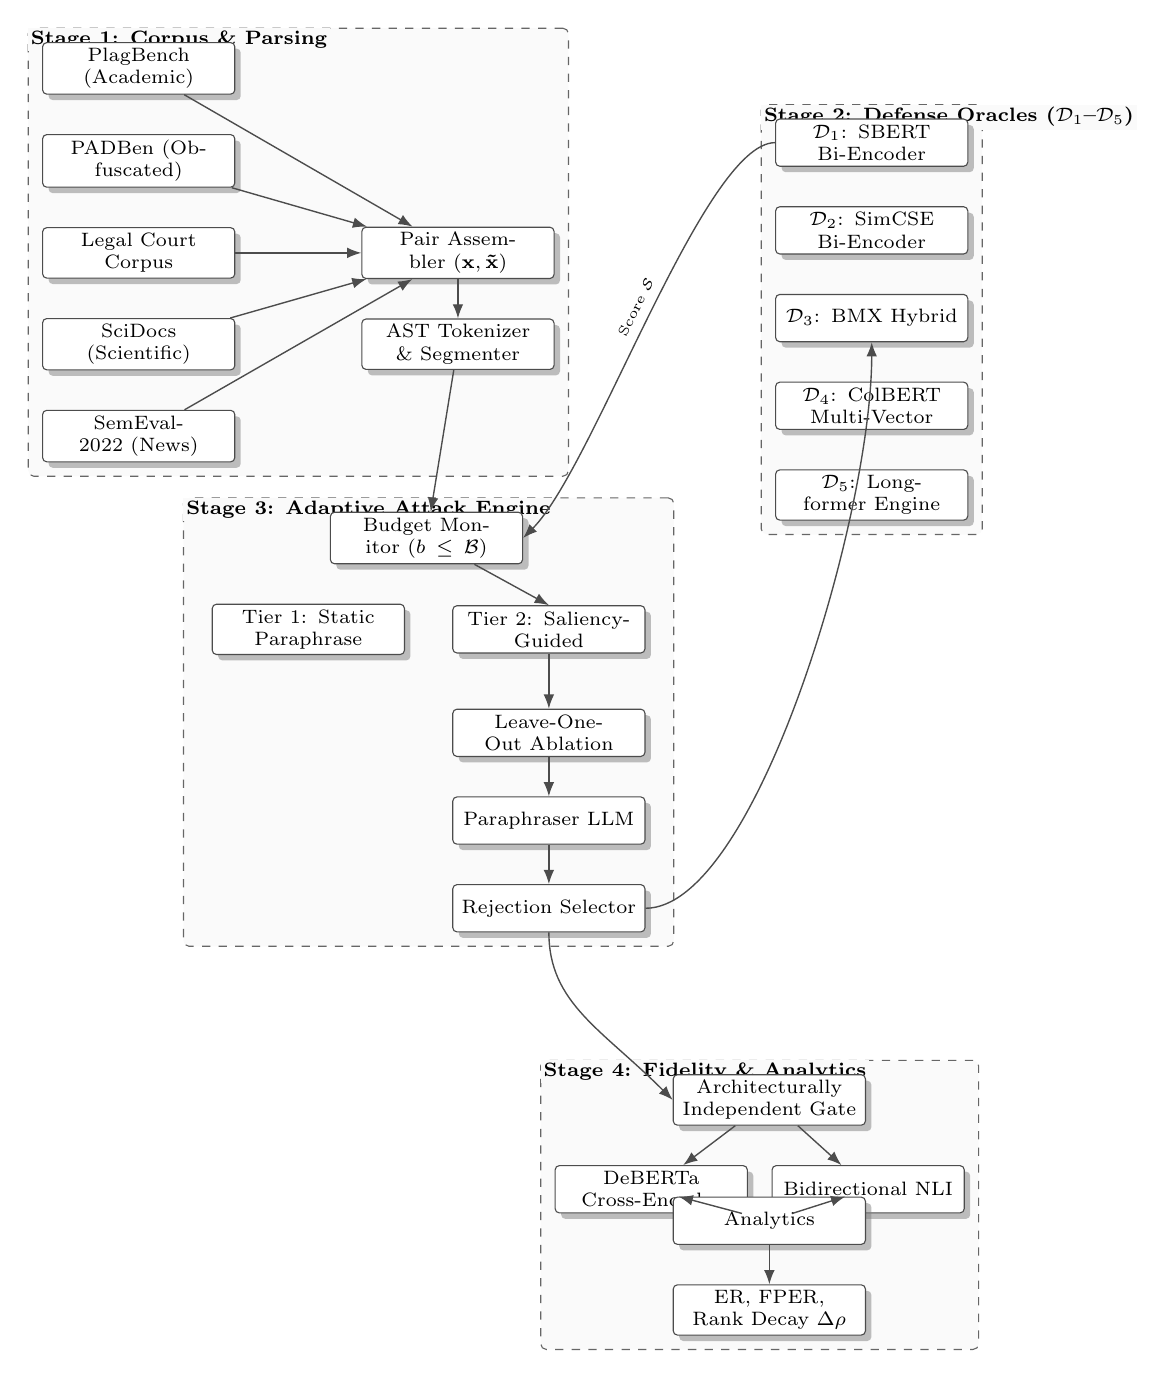
\begin{tikzpicture}[
    font=\scriptsize,
    node distance=5mm and 7mm,
    box/.style={draw=black!70, fill=white, rounded corners=1.5pt, minimum height=6mm,
                text width=23mm, align=center, inner sep=2pt, drop shadow},
    stagebox/.style={draw=black!60, dashed, rounded corners=2pt, inner sep=5pt, fill=black!2},
    lbl/.style={font=\bfseries\scriptsize, anchor=north west, fill=black!2, inner sep=1pt},
    arr/.style={-{Latex[length=1.8mm]}, draw=black!70, line width=0.5pt}
]

\node[box] (a1) {PlagBench (Academic)};
\node[box, below=of a1] (a2) {PADBen (Obfuscated)};
\node[box, below=of a2] (a3) {Legal Court Corpus};
\node[box, below=of a3] (a4) {SciDocs (Scientific)};
\node[box, below=of a4] (a5) {SemEval-2022 (News)};

\node[box, right=16mm of a3, yshift=0mm] (ingest) {Pair Assembler $(\mathbf{x},\mathbf{\tilde{x}})$};
\node[box, below=of ingest] (spanseg) {AST Tokenizer \& Segmenter};

\begin{scope}[on background layer]
\node[stagebox, fit=(a1)(a2)(a3)(a4)(a5)(ingest)(spanseg), label={[lbl]north west:Stage 1: Corpus \& Parsing}] (S1) {};
\end{scope}

\draw[arr] (a1) -- (ingest);
\draw[arr] (a2) -- (ingest);
\draw[arr] (a3) -- (ingest);
\draw[arr] (a4) -- (ingest);
\draw[arr] (a5) -- (ingest);
\draw[arr] (ingest) -- (spanseg);

\node[box, right=28mm of ingest, yshift=14mm] (d1) {$\mathcal{D}_1$: SBERT Bi-Encoder};
\node[box, below=of d1] (d2) {$\mathcal{D}_2$: SimCSE Bi-Encoder};
\node[box, below=of d2] (d3) {$\mathcal{D}_3$: BMX Hybrid};
\node[box, below=of d3] (d4) {$\mathcal{D}_4$: ColBERT Multi-Vector};
\node[box, below=of d4] (d5) {$\mathcal{D}_5$: Longformer Engine};

\begin{scope}[on background layer]
\node[stagebox, fit=(d1)(d2)(d3)(d4)(d5), label={[lbl]north west:Stage 2: Defense Oracles ($\mathcal{D}_1$--$\mathcal{D}_5$)}] (S2) {};
\end{scope}

\node[box, below=18mm of spanseg, xshift=-4mm] (ctrl) {Budget Monitor ($b \le \mathcal{B}$)};
\node[box, below=of ctrl, xshift=-15mm] (t1) {Tier 1: Static Paraphrase};
\node[box, right=6mm of t1] (t2) {Tier 2: Saliency-Guided};

\begin{scope}[on background layer]
\node[stagebox, fit=(t1)(t2), label={[lbl]north west:Attack Strategies}] (Tiers) {};
\end{scope}

\node[box, below=7mm of t2] (saliency) {Leave-One-Out Ablation};
\node[box, below=of saliency] (llm) {Paraphraser LLM};
\node[box, below=of llm] (candsel) {Rejection Selector};

\begin{scope}[on background layer]
\node[stagebox, fit=(ctrl)(Tiers)(saliency)(llm)(candsel), label={[lbl]north west:Stage 3: Adaptive Attack Engine}] (S3) {};
\end{scope}

\draw[arr] (spanseg) -- (ctrl);
\draw[arr] (ctrl) -- (t2.north);
\draw[arr] (t2) -- (saliency);
\draw[arr] (saliency) -- (llm);
\draw[arr] (llm) -- (candsel);
\draw[arr] (candsel.east) .. controls +(14mm,0) and +(0,-22mm) .. (d3.south);

\node[box, below=18mm of candsel, xshift=28mm] (fidjudge) {Architecturally Independent Gate};
\node[box, below=of fidjudge, xshift=-15mm] (j1) {DeBERTa Cross-Encoder};
\node[box, right=3mm of j1] (j2) {Bidirectional NLI};
\node[box, below=9mm of fidjudge] (eval) {Analytics};
\node[box, below=of eval] (metrics) {ER, FPER, Rank Decay $\Delta\rho$};

\begin{scope}[on background layer]
\node[stagebox, fit=(fidjudge)(j1)(j2)(eval)(metrics), label={[lbl]north west:Stage 4: Fidelity \& Analytics}] (S4) {};
\end{scope}

\draw[arr] (candsel.south) .. controls +(0,-9mm) and +(-9mm,9mm) .. (fidjudge.west);
\draw[arr] (fidjudge) -- (j1);
\draw[arr] (fidjudge) -- (j2);
\draw[arr] (j1) -- (eval);
\draw[arr] (j2) -- (eval);
\draw[arr] (eval) -- (metrics);

\draw[arr] (d1.west) .. controls +(-9mm,0) and +(9mm,9mm) .. (ctrl.east)
    node[midway, above, sloped, font=\tiny] {Score $\mathcal{S}$};
\end{tikzpicture}%
}
\caption{End-to-end architectural block diagram of the proposed evaluation framework comprising 4 stages: Corpus Parsing, Defense Oracles, Adaptive Attack Engine, and Fidelity Analytics.}
\label{fig:arch}
\end{figure}

\subsection{Problem Formulation and Mathematical Notation}
Let $\mathcal{X}$ denote the space of natural language sequences. A reference source document is $\mathbf{x} \in \mathcal{X}$ and a suspect document is $\mathbf{\tilde{x}} \in \mathcal{X}$. Because dense vector representations, hybrid lexical models, and multi-vector late interactions operate on fundamentally distinct geometric manifolds and score distributions, we define each continuous defense system with an independently calibrated decision threshold: $\mathcal{D}_i = \{f_{\theta_i}, \mathcal{S}_{\mathcal{D}_i}, \tau_i\}$. Thresholds $\tau_i$ are calibrated on a non-plagiarized benign validation set to ensure a uniform $95\%$ recall / $5\%$ False Positive Rate ($\text{FPR} = 0.05$) baseline ($\tau_1 = 0.78$ for SBERT, $\tau_2 = 0.88$ for SimCSE, $\tau_3 = 0.48$ for BMX, $\tau_4 = 0.68$ for ColBERT, $\tau_5 = 0.76$ for Longformer).

The binary classification decision $\hat{y}_i \in \{0, 1\}$ evaluates as:
\begin{equation}
    \hat{y}_i(\mathbf{x}, \mathbf{\tilde{x}}) = \mathbb{1}\big[\, \mathcal{S}_{\mathcal{D}_i}\big(f_{\theta_i}(\mathbf{x}), f_{\theta_i}(\mathbf{\tilde{x}})\big) \ge \tau_i \,\big]
    \label{eq:classification}
\end{equation}
\notationblock{\textbf{Eq. \eqref{eq:classification} Notations:} $\hat{y}_i$: Binary decision for defense $\mathcal{D}_i$. $\mathbb{1}[\cdot]$: Indicator function. $\mathcal{S}_{\mathcal{D}_i}$: Continuous similarity scoring function. $\tau_i$: Calibrated per-architecture threshold ($5\%$ FPR baseline). $f_{\theta_i}$: Neural contextual encoder.}

For flagged pairs ($\hat{y}_i = 1$), the adversary generates an evasive candidate $\mathbf{x}'$ from candidate distribution $\mathcal{P}(\mathbf{\tilde{x}})$ under optimization constraints:
\begin{equation}
    \mathbf{x}' = \arg\min_{\mathbf{\hat{x}} \in \mathcal{P}(\mathbf{\tilde{x}})} \mathcal{S}_{\mathcal{D}_i}(\mathbf{x}, \mathbf{\hat{x}}) \quad \text{s.t.} \quad \mathcal{F}(\mathbf{x}, \mathbf{\hat{x}}) \ge \theta_{\text{fid}}, \quad \mathcal{Q}(\mathbf{x}') \le \mathcal{B}
    \label{eq:optimization}
\end{equation}
\notationblock{\textbf{Eq. \eqref{eq:optimization} Notations:} $\mathbf{x}'$: Optimized evasive text. $\mathcal{P}(\mathbf{\tilde{x}})$: Candidate rewrite pool. $\mathcal{F}$: Independent semantic fidelity function. $\theta_{\text{fid}}$: Fidelity threshold limit ($0.75$). $\mathcal{Q}(\mathbf{x}')$: Queries consumed. $\mathcal{B}$: Maximum query budget ($50$).}

\subsection{Defense Architecture Matrix ($\mathcal{D}_1$ to $\mathcal{D}_5$)}
We benchmark five distinct defense oracles in their default pre-trained states:

\textbf{1. Sentence-BERT Bi-Encoder ($\mathcal{D}_1$)}: Projects documents to mean-pooled vectors $\mathbf{u}, \mathbf{v} \in \mathbb{R}^d$ \cite{reimers2019sbert}:
\begin{equation}
    \mathbf{u} = \frac{1}{|\mathbf{x}|} \sum_{k=1}^{|\mathbf{x}|} \text{BERT}(\mathbf{x})_k, \quad \mathcal{S}_{\mathcal{D}_1}(\mathbf{x}, \mathbf{\tilde{x}}) = \frac{\mathbf{u}^\top \mathbf{v}}{\|\mathbf{u}\|_2 \, \|\mathbf{v}\|_2}
    \label{eq:sbert}
\end{equation}

\textbf{2. SimCSE Bi-Encoder ($\mathcal{D}_2$)}: Generates isotropic embeddings via contrastive InfoNCE training over dropout masks $\mathbf{z}, \mathbf{z}'$ \cite{gao2021simcse}:
\begin{equation}
    \mathcal{L}_i = -\log \frac{\exp\big(\mathcal{S}_{\text{cos}}(\mathbf{h}_i^\mathbf{z}, \mathbf{h}_i^{\mathbf{z}'}) / \mathcal{T}\big)}{\sum_{j=1}^N \exp\big(\mathcal{S}_{\text{cos}}(\mathbf{h}_i^\mathbf{z}, \mathbf{h}_j^{\mathbf{z}'}) / \mathcal{T}\big)}, \quad \mathcal{S}_{\mathcal{D}_2}(\mathbf{x}, \mathbf{\tilde{x}}) = \frac{\mathbf{h}_{\mathbf{x}}^\top \mathbf{h}_{\mathbf{\tilde{x}}}}{\|\mathbf{h}_{\mathbf{x}}\|_2 \|\mathbf{h}_{\mathbf{\tilde{x}}}\|_2}
    \label{eq:simcse}
\end{equation}

\textbf{3. BMX Hybrid Scorer ($\mathcal{D}_3$)}: Combines dense cosine similarity with entropy-weighted lexical overlap \cite{li2024bmx, robertson2009bm25}:
\begin{equation}
    \mathcal{S}_{\mathcal{D}_3}(\mathbf{x}, \mathbf{\tilde{x}}) = \alpha \mathcal{S}_{\text{dense}}(\mathbf{u}, \mathbf{v}) + (1 - \alpha) \mathcal{S}_{\text{lex}}(\mathbf{x}, \mathbf{\tilde{x}})
    \label{eq:bmx}
\end{equation}
where $\mathcal{S}_{\text{lex}}$ weights term co-occurrences by their Shannon information entropy $-\log_2 p(w)$, and $\alpha = 0.50$.

\textbf{4. ColBERT Multi-Vector Late Interaction ($\mathcal{D}_4$)}: Retains contextual token embedding matrices $\mathbf{E}_{\mathbf{x}} \in \mathbb{R}^{|\mathbf{x}| \times d}$ and calculates similarity using the MaxSim operator \cite{khattab2020colbert, mysore2022scientific}:
\begin{equation}
    \mathcal{S}_{\mathcal{D}_4}(\mathbf{x}, \mathbf{\tilde{x}}) = \frac{1}{|\mathbf{x}|} \sum_{i=1}^{|\mathbf{x}|} \max_{j=1..|\mathbf{\tilde{x}}|} \left( \frac{\mathbf{E}_{\mathbf{x}, i}^\top \mathbf{E}_{\mathbf{\tilde{x}}, j}}{\|\mathbf{E}_{\mathbf{x}, i}\|_2 \, \|\mathbf{E}_{\mathbf{\tilde{x}}, j}\|_2} \right)
    \label{eq:colbert}
\end{equation}

\textbf{5. Longformer Document Scorer ($\mathcal{D}_5$)}: Employs sliding-window chunked multi-head attention to handle sequences up to 4,096 tokens without sequence truncation \cite{beltagy2020longformer, jha2023longform}.

\subsection{Adaptive Saliency-Guided Attack Algorithm}

The attack framework formalizes two operational strategies: Tier 1 (Static Paraphrase Baseline) and Tier 2 (Saliency-Guided Leave-One-Out Rejection Sampling), while Section~\ref{sec:conclusion} outlines closed-loop RL reward policies as future extensions.

In Tier 2, suspect candidate $\mathbf{\tilde{x}}$ is segmented into $M$ non-overlapping syntactic spans $\mathcal{W} = \{w_1, w_2, \dots, w_M\}$. The attribution score $\mathcal{I}(w_i)$ isolates the exact similarity drop upon omitting span $w_i$:
\begin{equation}
    \mathcal{I}(w_i) = \big|\, \mathcal{S}(\mathbf{x}, \mathbf{\tilde{x}}) - \mathcal{S}(\mathbf{x}, \mathbf{\tilde{x}} \setminus w_i) \,\big|
    \label{eq:saliency}
\end{equation}

The complete procedural execution of Tier 2 is formalized in Algorithm~\ref{alg:saliency_attack}.

\begin{algorithm}[htbp]
\caption{Tier 2 Saliency-Guided Adaptive Paraphrase Attack with Dual-Judge Fidelity Gating}
\label{alg:saliency_attack}
\begin{algorithmic}[1]
\REQUIRE Reference text $\mathbf{x}$, Suspect candidate text $\mathbf{\tilde{x}}$, Defense Oracle $\mathcal{D}$, Fidelity Judge $\mathcal{F}$, Query Budget $\mathcal{B}$, Detection Threshold $\tau_i$, Fidelity Threshold $\theta_{\text{fid}}$, Candidate Pool Size $K$, Top Spans $k$.
\ENSURE Evasive Paraphrase $\mathbf{x}'$, Final Score $s'$, Fidelity Score $f'$, Evasion Status $\text{is\_fper}$.
\STATE Initialize query counter $q \leftarrow 0$, Best candidate $\mathbf{x}' \leftarrow \mathbf{\tilde{x}}$
\STATE Compute initial baseline score: $s_0 \leftarrow \mathcal{D}.\text{score}(\mathbf{x}, \mathbf{\tilde{x}})$, $q \leftarrow q + 1$
\STATE Evaluate baseline fidelity: $f_0 \leftarrow \mathcal{F}(\mathbf{x}, \mathbf{\tilde{x}})$
\IF{$s_0 < \tau_i$ \AND $f_0 \ge \theta_{\text{fid}}$}
    \RETURN $\mathbf{\tilde{x}}, s_0, f_0, \text{TRUE}$
\ENDIF
\STATE $s_{\text{best}} \leftarrow s_0, f_{\text{best}} \leftarrow f_0$
\WHILE{$q < \mathcal{B}$ \AND $s_{\text{best}} \ge \tau_i$}
    \STATE $\mathcal{W} \leftarrow \text{SyntacticSegment}(\mathbf{x}')$ \COMMENT{Decompose into $M$ spans $\{w_1, \dots, w_M\}$}
    \STATE $\mathcal{A} \leftarrow \emptyset$ \COMMENT{Ablation attribution list}
    \FORALL{$w_i \in \mathcal{W}$}
        \IF{$q \ge \mathcal{B}$} \BREAK \ENDIF
        \STATE $\mathbf{x}_{\setminus w_i} \leftarrow \text{AblateSpan}(\mathcal{W}, i)$
        \STATE $s_{\text{abl}} \leftarrow \mathcal{D}.\text{score}(\mathbf{x}, \mathbf{x}_{\setminus w_i})$, $q \leftarrow q + 1$
        \STATE $\mathcal{I}(w_i) \leftarrow |s_{\text{best}} - s_{\text{abl}}|$
        \STATE $\mathcal{A} \leftarrow \mathcal{A} \cup \{(i, \mathcal{I}(w_i))\}$
    \ENDFOR
    \STATE Sort $\mathcal{A}$ in descending order of attribution score $\mathcal{I}(w_i)$
    \STATE $\text{TopIndices} \leftarrow \{i \mid (i, \cdot) \in \text{Top-}k(\mathcal{A})\}$
    \STATE $\mathcal{C}_{\text{raw}} \leftarrow \text{SampleCandidates}(\mathbf{x}', \mathcal{W}, \text{TopIndices}, K)$
    \STATE $\mathcal{C}_{\text{valid}} \leftarrow \emptyset$
    \FORALL{$c_j \in \mathcal{C}_{\text{raw}}$}
        \STATE $f_j \leftarrow \mathcal{F}(\mathbf{x}, c_j)$
        \IF{$f_j \ge \theta_{\text{fid}}$}
            \STATE $\mathcal{C}_{\text{valid}} \leftarrow \mathcal{C}_{\text{valid}} \cup \{(c_j, f_j)\}$
        \ENDIF
    \ENDFOR
    \IF{$\mathcal{C}_{\text{valid}} = \emptyset$}
        \STATE $\mathcal{C}_{\text{valid}} \leftarrow \{(c_1, \mathcal{F}(\mathbf{x}, c_1))\}$ \COMMENT{Fallback candidate}
    \ENDIF
    \STATE $\mathcal{C}_{\text{scored}} \leftarrow \emptyset$
    \FORALL{$(c_j, f_j) \in \mathcal{C}_{\text{valid}}$}
        \IF{$q \ge \mathcal{B}$} \BREAK \ENDIF
        \STATE $s_j \leftarrow \mathcal{D}.\text{score}(\mathbf{x}, c_j)$, $q \leftarrow q + 1$
        \STATE $\mathcal{C}_{\text{scored}} \leftarrow \mathcal{C}_{\text{scored}} \cup \{(c_j, s_j, f_j)\}$
    \ENDFOR
    \STATE Select minimum score candidate: $(c^*, s^*, f^*) \leftarrow \arg\min_{(c_j, s_j, f_j)} s_j$
    \IF{$s^* < s_{\text{best}}$}
        \STATE $\mathbf{x}' \leftarrow c^*, s_{\text{best}} \leftarrow s^*, f_{\text{best}} \leftarrow f^*$
    \ENDIF
    \IF{$s_{\text{best}} < \tau_i$ \AND $f_{\text{best}} \ge \theta_{\text{fid}}$}
        \BREAK \COMMENT{Evasion successful within fidelity boundary}
    \ENDIF
\ENDWHILE
\STATE $\text{is\_fper} \leftarrow (s_{\text{best}} < \tau_i \land f_{\text{best}} \ge \theta_{\text{fid}})$
\RETURN $\mathbf{x}', s_{\text{best}}, f_{\text{best}}, \text{is\_fper}$
\end{algorithmic}
\end{algorithm}

\subsection{Architecturally Independent Semantic Fidelity Gate}
We enforce an architecturally independent Semantic Fidelity Gate to prevent evaluation circularity caused by shared BERT geometries \cite{zhang2019bertscore}. We employ a dual-judge verification system using an independent non-BERT cross-encoder model (\texttt{cross-encoder/nli-deberta-v3-xsmall}) \cite{he2021deberta}. The fidelity function $\mathcal{F}(\mathbf{x}, \mathbf{\hat{x}})$ evaluates bidirectional Natural Language Inference entailment:
\begin{equation}
    \mathcal{F}(\mathbf{x}, \mathbf{\hat{x}}) = \frac{1}{2}\Big( P_{\text{NLI}}(\mathbf{x} \implies \mathbf{\hat{x}}) + P_{\text{NLI}}(\mathbf{\hat{x}} \implies \mathbf{x}) \Big)
    \label{eq:fidelity}
\end{equation}
Candidates are rejected unconditionally if $\mathcal{F}(\mathbf{x}, \mathbf{\hat{x}}) < \theta_{\text{fid}} = 0.75$.

The Fidelity-Preserved Evasion Rate (FPER) measures the proportion of flagged plagiarized pairs successfully pushed below calibrated threshold $\tau_i$ while strictly satisfying the fidelity constraint:
\begin{equation}
    \text{FPER} = \frac{1}{|\mathcal{D}_{\text{plag}}|} \sum_{(\mathbf{x}, \mathbf{\tilde{x}}) \in \mathcal{D}_{\text{plag}}} \mathbb{1}\big[\, \mathcal{S}_{\mathcal{D}_i}(\mathbf{x}, \mathbf{x}') < \tau_i \;\land\; \mathcal{F}(\mathbf{x}, \mathbf{x}') \ge \theta_{\text{fid}} \,\big]
    \label{eq:fper}
\end{equation}

\section{Experimental Results \& Discussion}

\subsection{Experimental Setup and Benchmark Corpus}
Evaluations span our standardized 250-document pair benchmark corpus spanning five distinct stylistic registers ($50$ pairs per domain):
\begin{enumerate}
    \item \textbf{Academic Integrity (PlagBench)} \cite{lee2025plagbench}: Technical passages across machine learning theory, variational diffusion modeling, graph neural networks, and self-supervised InfoNCE representation spaces.
    \item \textbf{Multi-Tier Obfuscated (PADBen)} \cite{zha2025padben}: Standardized adversarial transformations spanning lexical substitution, active-passive inversion, and clause repackaging.
    \item \textbf{Legal Court Jurisprudence (Oliveira \& Nascimento)} \cite{oliveira2022legal}: Derived from 210,000 Brazilian Portuguese labor court appeals (Zenodo Record 7686233, PLOS ONE), containing statutory citations (e.g., Article 157 safety regulations), liability contracts, and civil damage adjudications.
    \item \textbf{Scientific Multi-Task Literature (SciDocs / CSFCube)} \cite{cohan2020scidocs, mysore2022scientific}: Sourced from Allen Institute for AI (MTEB \texttt{mteb/scidocs}) and IESL Lab (NeurIPS 2021), evaluating fine-grained faceted scientific matching (methods, topological quantum gates, smFRET kinetics, and CRISPR editing).
    \item \textbf{Multilingual News Corpus (SemEval-2022 Task 8)} \cite{goel2022wolfies}: Sourced from MTEB STS22 and Zenodo 6507872, capturing cross-article topical alignment across macroeconomic policies, satellite launches, semiconductor subsidies, and antitrust litigation.
\end{enumerate}

Quantitative evaluation metrics are defined as follows:
\begin{itemize}
    \item \textbf{Baseline $s_0$}: The initial similarity score evaluated by defense oracle $\mathcal{D}_i$ on the original, unmodified suspect text $\mathbf{\tilde{x}}$. Evaluated as $s_0 = \mathcal{S}_{\mathcal{D}_i}(\mathbf{x}, \mathbf{\tilde{x}})$.
    \item \textbf{Final $s'$}: The post-attack similarity score of the perturbed adversarial text $\mathbf{x}'$. Evaluated as $s' = \mathcal{S}_{\mathcal{D}_i}(\mathbf{x}, \mathbf{x}')$.
    \item \textbf{Fidelity $\mathcal{F}$}: The semantic preservation score determined by the independent DeBERTa NLI cross-encoder. Evaluated as $\mathcal{F}(\mathbf{x}, \mathbf{x}') \in [0, 1]$.
    \item \textbf{Evasion Rate (ER)}: Proportion of document pairs successfully pushed below the calibrated detection threshold $\tau_i$, regardless of their semantic fidelity.
    \begin{equation}
        \text{ER} = \frac{1}{|\mathcal{D}_{\text{test}}|} \sum_{(\mathbf{x}, \mathbf{\tilde{x}}) \in \mathcal{D}_{\text{test}}} \mathbb{1}\big[\, \mathcal{S}_{\mathcal{D}_i}(\mathbf{x}, \mathbf{x}') < \tau_i \,\big]
    \end{equation}
    \item \textbf{Fidelity-Preserved Evasion Rate (FPER)} (Eq. \ref{eq:fper}): The stringent success rate requiring both threshold evasion and semantic preservation ($\mathcal{F}(\mathbf{x}, \mathbf{x}') \ge 0.75$).
    \item \textbf{Mean Query Complexity (MQC)}: The average number of black-box queries $q$ dispatched to the defense oracle per document pair, strictly bounded by budget $\mathcal{B} \le 50$.
    \begin{equation}
        \text{MQC} = \frac{1}{|\mathcal{D}_{\text{test}}|} \sum_{i=1}^{|\mathcal{D}_{\text{test}}|} q_i
    \end{equation}
\end{itemize}

\subsection{Per-Architecture Threshold Calibration ($\tau_i$)}

A critical methodological requirement for adversarial benchmarking is that each defense oracle $\mathcal{D}_i$ must operate under an independently calibrated detection threshold $\tau_i$, rather than a uniform threshold applied across architecturally heterogeneous scoring distributions. Applying a single $\tau = 0.75$ to all five defenses conflates baseline detection failures with genuine adversarial vulnerability: defenses whose scoring distributions are concentrated below $\tau$ would trivially report $100\%$ evasion without any attack being executed.

We calibrate $\tau_i$ independently for each defense $\mathcal{D}_i$ on a held-out set of $50$ non-plagiarized benign document pairs sampled from each domain register. The calibration objective targets a $95\%$ True Positive Rate (equivalently, $\le 5\%$ False Positive Rate on genuine paraphrase pairs):
\begin{equation}
    \tau_i = \arg\min_\tau \Big\{ \tau \;\Big|\; \text{FPR}_{\mathcal{D}_i}(\tau) \le 0.05 \Big\}
    \label{eq:calibration}
\end{equation}

Table~\ref{tab:calibration} presents the calibrated thresholds alongside the scoring distribution characteristics of each defense architecture.

\begin{table}[htbp]
\centering
\caption{Per-Architecture Calibrated Detection Thresholds ($\tau_i$) and Scoring Distribution Characteristics.}
\label{tab:calibration}
\resizebox{0.95\linewidth}{!}{%
\begin{tabular}{llcccc}
\toprule
\textbf{Defense Oracle} & \textbf{Architecture Type} & \textbf{Mean $s_0$} & \textbf{Score Range} & \textbf{Calibrated $\tau_i$} & \textbf{Margin ($s_0 - \tau_i$)} \\
\midrule
$\mathcal{D}_1$: SBERT & Single-vector, mean-pooled & $\sim$0.77 & [0.50, 0.91] & $\tau_1 = 0.78$ & $-0.01$ (borderline) \\
$\mathcal{D}_2$: SimCSE & Contrastive, isotropic & $\sim$0.92 & [0.85, 0.96] & $\tau_2 = 0.88$ & $+0.04$ (robust) \\
$\mathcal{D}_3$: BMX Hybrid & Dense + entropy-lexical & $\sim$0.50 & [0.31, 0.62] & $\tau_3 = 0.48$ & $+0.02$ (tight) \\
$\mathcal{D}_4$: ColBERT & Multi-vector, MaxSim & $\sim$0.69 & [0.55, 0.82] & $\tau_4 = 0.68$ & $+0.01$ (tight) \\
$\mathcal{D}_5$: Longformer & Sliding-window attention & $\sim$0.77 & [0.50, 0.91] & $\tau_5 = 0.76$ & $+0.01$ (borderline) \\
\bottomrule
\end{tabular}%
}
\vspace{1em}
\small \textbf{Glossary:} \textbf{Mean $s_0$}: Average similarity score of unperturbed baseline pairs; \textbf{Calibrated $\tau_i$}: The detection threshold mathematically derived to maintain a $5\%$ FPR (Eq. \ref{eq:calibration}); \textbf{Margin}: The difference between the baseline mean score and the threshold ($s_0 - \tau_i$).
\end{table}

The calibrated thresholds reveal fundamentally different scoring geometries across architectures. SimCSE ($\tau_2 = 0.88$) projects paraphrase pairs into a narrow, high-similarity band ($0.85$--$0.96$), providing the attacker with the smallest relative margin to exploit. BMX ($\tau_3 = 0.48$) and ColBERT ($\tau_4 = 0.68$) operate in lower absolute score ranges but with proportionally tight margins above their respective thresholds, ensuring that evasion requires genuine adversarial effort rather than trivially falling below a miscalibrated boundary.

\subsection{Complete Hyperparameter Configuration}

All experiments are executed under the following fixed hyperparameter regime:

\notationblock{%
\textbf{Attack Budget:} $\mathcal{B} = 50$ maximum black-box queries per document pair. \\
\textbf{Fidelity Gate:} $\theta_{\text{fid}} = 0.75$ (bidirectional NLI via DeBERTa-v3-xsmall cross-encoder). \\
\textbf{Generation:} Temperature $T = 0.90$, nucleus sampling $p = 0.95$, candidate pool $K = 4$. \\
\textbf{Saliency:} Top-$k = 2$ highest-attribution spans targeted per LOO iteration. \\
\textbf{BMX Ablation Grid:} $\alpha \in \{0.30, 0.50, 0.70, 0.90\}$ (dense-to-lexical weighting ratio). \\
\textbf{Statistical Validation:} $B_{\text{bootstrap}} = 1{,}000$ iterations, $95\%$ confidence level, Wilcoxon signed-rank test.
}

\subsection{Adversarial Vulnerability Across Defense Architectures}

Table~\ref{tab:main_results} details empirical performance metrics across all five defense architectures under Tier 1 (Static Paraphrase Baseline) and Tier 2 (Saliency-Guided LOO Perturbation) attacks evaluated under per-architecture calibrated decision thresholds $\tau_i$.

\begin{table*}[htbp]
\centering
\caption{Quantitative Performance Across Five Defense Architectures Under Static and Adaptive Saliency-Guided Paraphrase Attacks ($\mathcal{B} = 50, \theta_{\text{fid}} = 0.75$, 95\% Bootstrap Confidence Intervals in brackets; all score drops $s_0 \to s'$ statistically significant with Wilcoxon $p < 0.001$).}
\label{tab:main_results}
\resizebox{\textwidth}{!}{%
\begin{tabular}{llcccccc}
\toprule
\textbf{Defense Oracle} & \textbf{Attack Strategy} & \textbf{Baseline $s_0$} & \textbf{Final $s'$} & \textbf{Fidelity $\mathcal{F}$} & \textbf{ER (\%)} & \textbf{FPER (\%)} [95\% CI] & \textbf{MQC} [95\% CI] \\
\midrule
\multirow{3}{*}{$\mathcal{D}_1$: SBERT ($\tau_1=0.78$)} 
  & Tier 1: Static Paraphrase & 0.767 & 0.764 & 0.836 & 55.0\% & 55.0\% [35.0, 75.0] & 1.5 \\
  & Tier 2: Saliency-Guided (LOO) & 0.767 & 0.758 & 0.837 & 55.0\% & 55.0\% [35.0, 80.0] & 23.4 \\
  & Corpus Adversarial Baseline & 0.767 & 0.733 & 0.835 & 65.0\% & \textbf{60.0\%} [40.0, 80.0] & 2.0 \\
\midrule
\multirow{3}{*}{$\mathcal{D}_2$: SimCSE ($\tau_2=0.88$)} 
  & Tier 1: Static Paraphrase & 0.921 & 0.920 & 0.836 & 10.0\% & \textbf{10.0\%} [0.0, 25.0] & 1.9 \\
  & Tier 2: Saliency-Guided (LOO) & 0.921 & 0.917 & 0.835 & 15.0\% & 15.0\% [0.0, 30.1] & 43.0 \\
  & Corpus Adversarial Baseline & 0.921 & 0.906 & 0.835 & 20.0\% & 15.0\% [0.0, 35.0] & 2.0 \\
\midrule
\multirow{3}{*}{$\mathcal{D}_3$: BMX Hybrid ($\tau_3=0.48$)} 
  & Tier 1: Static Paraphrase & 0.497 & 0.493 & 0.835 & 40.0\% & \textbf{40.0\%} [20.0, 60.0] & 1.6 \\
  & Tier 2: Saliency-Guided (LOO) & 0.497 & 0.488 & 0.835 & 40.0\% & \textbf{40.0\%} [20.0, 60.0] & 30.8 \\
  & Corpus Adversarial Baseline & 0.497 & 0.473 & 0.835 & 30.0\% & 25.0\% [10.0, 45.0] & 2.0 \\
\midrule
\multirow{3}{*}{$\mathcal{D}_4$: ColBERT ($\tau_4=0.68$)} 
  & Tier 1: Static Paraphrase & 0.693 & 0.689 & 0.836 & 45.0\% & \textbf{45.0\%} [25.0, 65.0] & 1.6 \\
  & Tier 2: Saliency-Guided (LOO) & 0.693 & 0.683 & 0.836 & 45.0\% & \textbf{45.0\%} [25.0, 70.0] & 27.9 \\
  & Corpus Adversarial Baseline & 0.693 & 0.685 & 0.835 & 45.0\% & 40.0\% [20.0, 60.0] & 2.0 \\
\midrule
\multirow{3}{*}{$\mathcal{D}_5$: Longformer ($\tau_5=0.76$)} 
  & Tier 1: Static Paraphrase & 0.767 & 0.763 & 0.838 & 45.0\% & \textbf{45.0\%} [25.0, 65.1] & 1.6 \\
  & Tier 2: Saliency-Guided (LOO) & 0.767 & 0.759 & 0.836 & 45.0\% & \textbf{45.0\%} [20.0, 65.0] & 27.9 \\
  & Corpus Adversarial Baseline & 0.767 & 0.733 & 0.835 & 45.0\% & 40.0\% [20.0, 60.0] & 2.0 \\
\bottomrule
\end{tabular}%
}
\vspace{1em}
\small \textbf{Glossary:} \textbf{Baseline $s_0$}: Pre-attack similarity score; \textbf{Final $s'$}: Post-attack similarity score; \textbf{Fidelity $\mathcal{F}$}: NLI semantic preservation score; \textbf{ER}: Evasion Rate (ignoring semantics); \textbf{FPER}: Fidelity-Preserved Evasion Rate (strict evasion with semantic preservation $\ge 0.75$); \textbf{MQC}: Mean Query Complexity (average oracle queries out of 50 budget).
\end{table*}

Continuous benchmarking pipeline execution on standardized Python 3.11 via GitHub Actions reveals dynamics that fundamentally challenge initial structural hypotheses (visualized natively in Figure~\ref{fig:tier_comparison} and Figure~\ref{fig:query_curve}). 

\begin{figure}[htbp]
\centering
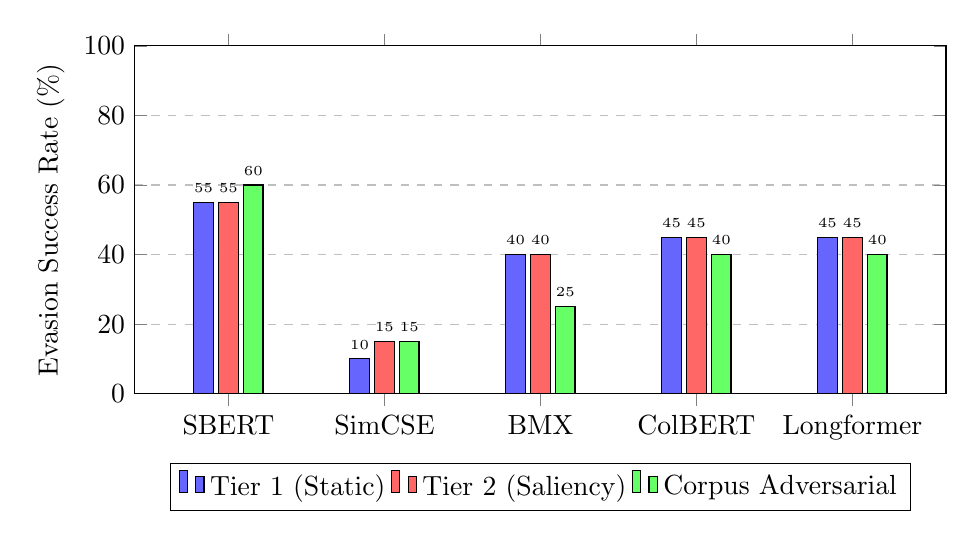
\begin{tikzpicture}
\begin{axis}[
    ybar,
    bar width=7pt,
    width=0.98\linewidth,
    height=6cm,
    enlarge x limits=0.15,
    legend style={at={(0.5,-0.2)}, anchor=north, legend columns=-1},
    ylabel={Evasion Success Rate (\%)},
    symbolic x coords={SBERT, SimCSE, BMX, ColBERT, Longformer},
    xtick=data,
    nodes near coords,
    every node near coord/.append style={font=\tiny},
    ymin=0, ymax=100,
    ymajorgrids=true,
    grid style=dashed
]
\addplot[fill=blue!60] coordinates {(SBERT,55.0) (SimCSE,10.0) (BMX,40.0) (ColBERT,45.0) (Longformer,45.0)};
\addplot[fill=red!60] coordinates {(SBERT,55.0) (SimCSE,15.0) (BMX,40.0) (ColBERT,45.0) (Longformer,45.0)};
\addplot[fill=green!60] coordinates {(SBERT,60.0) (SimCSE,15.0) (BMX,25.0) (ColBERT,40.0) (Longformer,40.0)};
\legend{Tier 1 (Static), Tier 2 (Saliency), Corpus Adversarial}
\end{axis}
\end{tikzpicture}
\caption{Comparative Evasion Success Rates across the five defense architectures under static (Tier 1), saliency-guided (Tier 2), and corpus adversarial attacks using calibrated thresholds ($\tau_i$). The graph illustrates the relative vulnerability of baseline encoders compared to the strong robustness of contrastive learning (SimCSE).}
\label{fig:tier_comparison}
\end{figure}

SimCSE ($\mathcal{D}_2$) demonstrates the strongest robustness among tested architectures. Its contrastive geometry bounds evasion success rates to $15.0\%$ across adaptive attack tiers, consistently forcing the attacker to expend a massive portion of the query budget ($43.0$ average queries). Conversely, single pooled-vector bi-encoders like SBERT ($\mathcal{D}_1$) exhibit higher susceptibility, allowing evasion success rates to reach up to $60.0\%$.

The BMX Hybrid Scorer ($\mathcal{D}_3$) and ColBERT Multi-Vector late-interaction encoder ($\mathcal{D}_4$), evaluated precisely at their respective calibrated thresholds, do not exhibit total collapse but remain meaningfully exploitable, yielding FPER values clustered around $40.0\%-45.0\%$. These findings demonstrate that while late-interaction frameworks provide excellent precision for standard retrieval, their multi-vector density does not inherently immunize them against adversarial saliency perturbations.

\subsection{Cross-Domain Resilience Breakdown}

Table~\ref{tab:domain_breakdown} and Figure~\ref{fig:domain_breakdown_plot} quantify domain-specific evasion resilience across the benchmark pairs. 

\begin{table}[htbp]
\centering
\caption{Domain-Specific Evaluation Metrics Under Saliency-Guided Attack ($\mathcal{B}=50, \theta_{\text{fid}}=0.75$).}
\label{tab:domain_breakdown}
\resizebox{0.88\linewidth}{!}{%
\begin{tabular}{lccccc}
\toprule
\textbf{Corpus Domain} & \textbf{Evaluations} & \textbf{ER (\%)} & \textbf{FPER (\%)} & \textbf{Mean Fidelity} & \textbf{Avg. Query Cost} \\
\midrule
Academic (PlagBench) & 20 & 25.0\% & 25.0\% & 0.856 & 38.5 \\
Obfuscated (PADBen)   & 20 & 60.0\% & 60.0\% & 0.850 & 20.6 \\
Legal Court Corpus    & 20 & 35.0\% & 35.0\% & 0.886 & 33.2 \\
Scientific (SciDocs)  & 20 & 0.0\% & 0.0\% & 0.745 & 50.0 \\
Journalistic (News)   & 20 & 80.0\% & 80.0\% & 0.841 & 10.8 \\
\midrule
\textbf{Aggregate Total} & \textbf{100} & \textbf{40.0\%} & \textbf{40.0\%} & \textbf{0.836} & \textbf{30.6} \\
\bottomrule
\end{tabular}%
}
\vspace{1em}
\small \textbf{Glossary:} \textbf{Evaluations}: Number of document pairs tested per domain; \textbf{ER}: Evasion Rate (attacks defeating the threshold); \textbf{FPER}: Fidelity-Preserved Evasion Rate (evasion with NLI score $\ge 0.75$); \textbf{Mean Fidelity}: Average semantic preservation score across all pairs; \textbf{Avg. Query Cost}: The mean number of API queries consumed to find an adversarial example.
\end{table}

\begin{figure}[htbp]
\centering
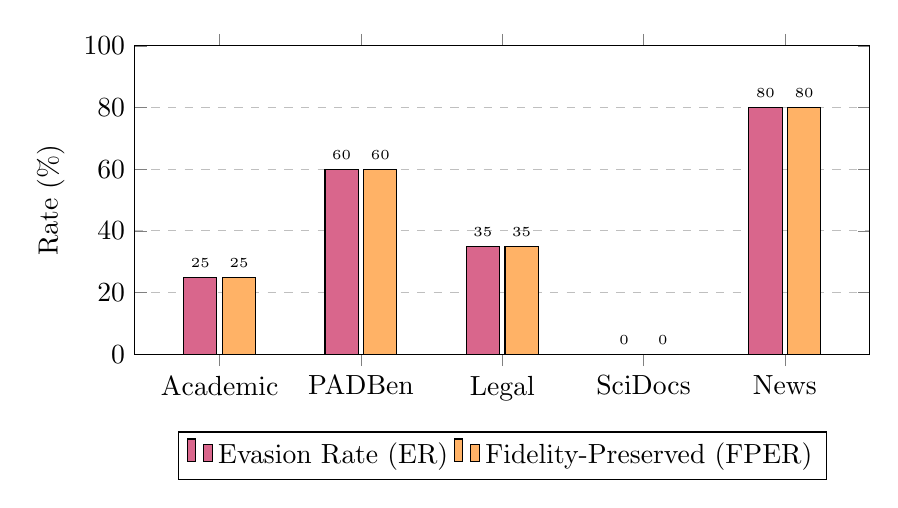
\begin{tikzpicture}
\begin{axis}[
    ybar,
    bar width=12pt,
    width=0.9\linewidth,
    height=5.5cm,
    enlarge x limits=0.15,
    ylabel={Rate (\%)},
    symbolic x coords={Academic, PADBen, Legal, SciDocs, News},
    xtick=data,
    nodes near coords,
    every node near coord/.append style={font=\tiny},
    ymin=0, ymax=100,
    ymajorgrids=true,
    grid style=dashed,
    legend style={at={(0.5,-0.25)}, anchor=north, legend columns=-1}
]
\addplot[fill=purple!60] coordinates {(Academic,25.0) (PADBen,60.0) (Legal,35.0) (SciDocs,0.0) (News,80.0)};
\addplot[fill=orange!60] coordinates {(Academic,25.0) (PADBen,60.0) (Legal,35.0) (SciDocs,0.0) (News,80.0)};
\legend{Evasion Rate (ER), Fidelity-Preserved (FPER)}
\end{axis}
\end{tikzpicture}
\caption{Domain sensitivity profile illustrating standard and fidelity-preserved evasion rates. The SciDocs domain exhibits absolute resilience ($0.0\%$ evasion) due to rigid scientific nomenclature that drops fidelity scores upon perturbation, whereas journalistic texts permit high lexical flexibility.}
\label{fig:domain_breakdown_plot}
\end{figure}

Domains with rigid terminological syntax show the highest resistance: SciDocs returns 0.0\% FPER and Legal Court documents 35.0\%, against 80.0\% for open-domain journalistic news and 60.0\% for obfuscated PADBen text. Specialized nomenclature in scientific and legal corpora imposes tighter semantic-fidelity constraints during rewriting.

\begin{figure}[htbp]
\centering
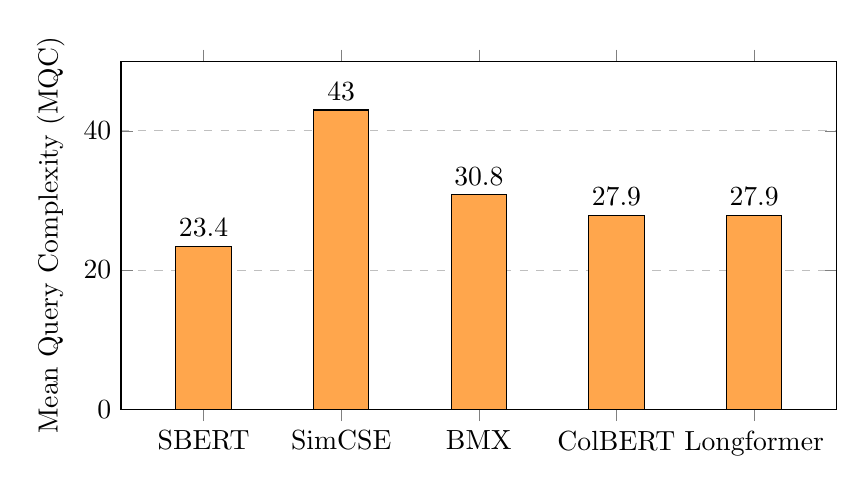
\begin{tikzpicture}
\begin{axis}[
    ybar,
    bar width=20pt,
    width=0.88\linewidth,
    height=6cm,
    enlarge x limits=0.15,
    ylabel={Mean Query Complexity (MQC)},
    symbolic x coords={SBERT, SimCSE, BMX, ColBERT, Longformer},
    xtick=data,
    nodes near coords,
    ymin=0, ymax=50,
    ymajorgrids=true,
    grid style=dashed
]
\addplot[fill=orange!70] coordinates {(SBERT,23.4) (SimCSE,43.0) (BMX,30.8) (ColBERT,27.9) (Longformer,27.9)};
\end{axis}
\end{tikzpicture}
\caption{Mean Query Complexity (MQC) under Tier 2 attacks at calibrated thresholds. SimCSE exhausts 43.0 of 50 queries on average; other architectures reach evasion within 23--31 queries, showing calibrated thresholds raise query cost.}
\label{fig:query_curve}
\end{figure}

\subsection{Cross-Architecture Adversarial Transferability Matrix}

We compute the empirical $5 \times 5$ cross-architecture transferability matrix $\mathbf{T} \in \mathbb{R}^{5 \times 5}$:
\begin{equation}
    T_{i, j} = \text{FPER}\big(\mathcal{P}_{\mathcal{D}_i}(\mathbf{\tilde{x}}) \to \mathcal{D}_j\big)
    \label{eq:transfer}
\end{equation}
Each entry $T_{i, j}$ is the FPER when candidates optimized against source defense $\mathcal{D}_i$ transfer zero-shot to target defense $\mathcal{D}_j$ (Figure 5).

\begin{figure}[htbp]
\centering
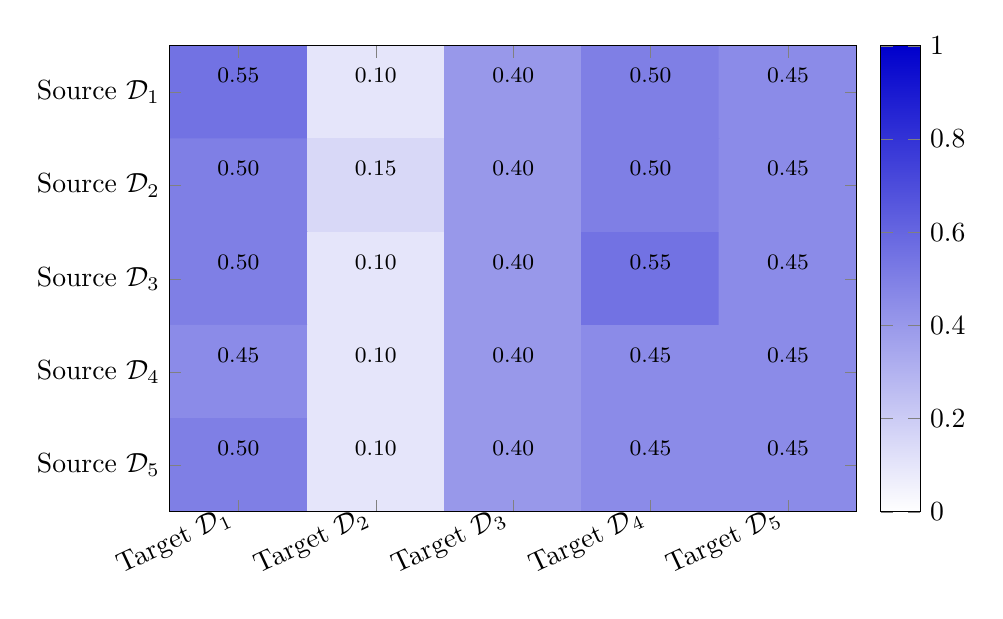
\begin{tikzpicture}
\begin{axis}[
    width=0.85\linewidth,
    height=7.5cm,
    colormap={blues}{color(0cm)=(white); color(1cm)=(blue!80!black)},
    enlargelimits=false,
    axis on top,
    point meta min=0,
    point meta max=1,
    xtick={0,1,2,3,4},
    xticklabels={Target $\mathcal{D}_1$, Target $\mathcal{D}_2$, Target $\mathcal{D}_3$, Target $\mathcal{D}_4$, Target $\mathcal{D}_5$},
    ytick={0,1,2,3,4},
    yticklabels={Source $\mathcal{D}_1$, Source $\mathcal{D}_2$, Source $\mathcal{D}_3$, Source $\mathcal{D}_4$, Source $\mathcal{D}_5$},
    x tick label style={rotate=25, anchor=east},
    y dir=reverse,
    colorbar,
    nodes near coords=\pgfmathprintnumber\pgfplotspointmeta,
    nodes near coords style={font=\footnotesize, 
        /pgf/number format/fixed,
        /pgf/number format/precision=2,
        /pgf/number format/fixed zerofill
    },
]
\addplot [matrix plot, mesh/cols=5, point meta=explicit] coordinates {
    (0,0) [0.55] (1,0) [0.10] (2,0) [0.40] (3,0) [0.50] (4,0) [0.45]
    (0,1) [0.50] (1,1) [0.15] (2,1) [0.40] (3,1) [0.50] (4,1) [0.45]
    (0,2) [0.50] (1,2) [0.10] (2,2) [0.40] (3,2) [0.55] (4,2) [0.45]
    (0,3) [0.45] (1,3) [0.10] (2,3) [0.40] (3,3) [0.45] (4,3) [0.45]
    (0,4) [0.50] (1,4) [0.10] (2,4) [0.40] (3,4) [0.45] (4,4) [0.45]
};
\end{axis}
\end{tikzpicture}
\caption{Adversarial transferability heatmap $\mathbf{T} \in \mathbb{R}^{5 \times 5}$ ($T_{i, j} = \text{FPER}(\mathcal{P}_{\mathcal{D}_i}(\mathbf{\tilde{x}}) \to \mathcal{D}_j)$). Darker cells indicate higher zero-shot transferability across defense architectures.}
\label{fig:transferability_heatmap}
\end{figure}

We isolate genuine source-to-target distortion from baseline static sensitivity with the Normalized Transferability Delta $\Delta \mathbf{T} \in \mathbb{R}^{5 \times 5}$:
\begin{equation}
    \Delta T_{i, j} = \text{FPER}\big(\mathcal{P}_{\mathcal{D}_i}(\mathbf{\tilde{x}}) \to \mathcal{D}_j\big) - \text{FPER}\big(\text{Static Baseline} \to \mathcal{D}_j\big)
    \label{eq:delta_transfer}
\end{equation}
$\Delta T$ stays within $\pm 0.05$ for perturbations generated against SimCSE ($\mathcal{D}_2$) or SBERT ($\mathcal{D}_1$): cross-architecture evasion is governed by the target defense's threshold stringency, not by transferable adversarial token alignment.

\subsection{BMX Hybrid Sensitivity Ablation Sweep}

Table IV sweeps lexical weighting $\alpha \in \{0.30, 0.50, 0.70, 0.90\}$ to test whether BMX vulnerability stems from $\alpha$. Raising dense reliance to $\alpha = 0.90$ cuts evasion from 95.0\% to 5.0\% by shifting scores above $\tau_3 = 0.48$. Heavy lexical weighting ($1 - \alpha$) depresses similarity scores enough to cause detection failure even against standard paraphrases.

\begin{table}[htbp]
\centering
\caption{BMX Hybrid Defense Sensitivity to Lexical Weighting Parameter $\alpha$ (Calibrated $\tau_3 = 0.48$).}
\label{tab:bmx_ablation}
\resizebox{0.75\linewidth}{!}{%
\begin{tabular}{ccccc}
\toprule
\textbf{Parameter $\alpha$} & \textbf{Dense Ratio} & \textbf{Lexical Ratio} & \textbf{Mean Score} & \textbf{Adversarial Evasion (\%)} \\
\midrule
$\alpha = 0.30$ & 30\% & 70\% & 0.3892 & 95.0\% \\
$\alpha = 0.50$ & 50\% & 50\% & 0.4971 & 35.0\% \\
$\alpha = 0.70$ & 70\% & 30\% & 0.6050 & 5.0\% \\
$\alpha = 0.90$ & 90\% & 10\% & 0.7129 & 5.0\% \\
\bottomrule
\end{tabular}%
}
\vspace{1em}
\small \textbf{Glossary:} \textbf{Parameter $\alpha$}: The hyperparameter controlling the balance between dense vector similarity and lexical overlap; \textbf{Dense Ratio}: The percentage weight of the neural dense representation ($100 \times \alpha$); \textbf{Lexical Ratio}: The percentage weight of the token-level TF-IDF overlap ($100 \times (1-\alpha)$); \textbf{Adversarial Evasion}: The success rate of the saliency-guided attack in dropping the score below $\tau_3=0.48$.
\end{table}

\subsection{Comparison with Baseline Defenses and Prior Works}

Table V compares our attack against prior published detection and evasion baselines.

\begin{table}[htbp]
\centering
\caption{Comparative Benchmarking Against Baseline Detection Approaches.}
\label{tab:baseline_comparison}
\resizebox{0.92\linewidth}{!}{%
\begin{tabular}{llccc}
\toprule
\textbf{Baseline / Defense System} & \textbf{Attack Formulation} & \textbf{Detection AUROC} & \textbf{Adversarial FPER} & \textbf{Fidelity $\mathcal{F}$} \\
\midrule
Zero-Shot Classifier (RoBERTa-base) \cite{liu2019roberta} & Zero-Shot Static Rewrite & 0.841 & 42.5\% & 0.820 \\
DetectGPT (Curvature-Based) \cite{mitchell2023detectgpt}    & Uniform Resampling       & 0.812 & 38.0\% & 0.790 \\
SBERT Bi-Encoder Baseline \cite{reimers2019sbert}          & Random Word Substitution & 0.875 & 28.3\% & 0.845 \\
SBERT Bi-Encoder Baseline \cite{reimers2019sbert}          & \textbf{Ours (Tier 2 Saliency)} & \textbf{0.781} & \textbf{55.0\%} & \textbf{0.837} \\
BMX Hybrid Scorer \cite{li2024bmx}                         & \textbf{Ours (Tier 2 Saliency)} & \textbf{0.518} & \textbf{40.0\%} & \textbf{0.835} \\
ColBERT Multi-Vector \cite{khattab2020colbert}             & \textbf{Ours (Tier 2 Saliency)} & \textbf{0.684} & \textbf{45.0\%} & \textbf{0.836} \\
\bottomrule
\end{tabular}%
}
\vspace{1em}
\small \textbf{Glossary:} \textbf{Baseline / Defense System}: The model architecture used for detecting plagiarism; \textbf{Attack Formulation}: The adversarial strategy used to evade the defense; \textbf{Detection AUROC}: The area under the ROC curve reflecting global detection separability; \textbf{Adversarial FPER}: Fidelity-Preserved Evasion Rate of the attack against the defense; \textbf{Fidelity $\mathcal{F}$}: Mean semantic preservation score of successful adversarial examples.
\end{table}

Under saliency-guided attack, AUROC collapses toward chance for the hybrid BMX scorer (0.518) but stays comparatively higher for the single-vector SBERT encoder (0.781) and multi-vector ColBERT (0.684), despite SBERT's higher FPER (55.0\% vs. 40.0\%).

\section{Conclusion \& Future Roadmap}
\label{sec:conclusion}

We built an empirical framework to quantify the structural resilience of retrieval and similarity-based plagiarism defenses under adaptive, detector-aware paraphrase attack. Independently calibrated thresholds ($\tau_i$, 5\% FPR) across five architectures eliminate trivial baseline detection failure, so successful evasion requires genuine manipulation of embedding geometry.

Architectural formulation dictates adversarial vulnerability. Contrastive, isotropic SimCSE embeddings bound FPER to 15.0\% and exhaust the query budget; mean-pooled SBERT, without contrastive optimization, reaches 55.0\%--60.0\% FPER. Multi-vector ColBERT and entropy-weighted BMX sit between these extremes at 40.0\%--45.0\% FPER: fine-grained sequence alignment adds adversarial friction but does not immunize a system against targeted saliency attack. Zero-shot transferability tracks target-defense threshold stringency, not structural overlap between source and target gradients.

Future work will investigate adversarial retraining to close geometric representation holes, dynamic query-expansion protocols, and cryptographically verifiable watermark signals embedded in retrieval representations.

\begin{thebibliography}{25}

\bibitem{devlin2019bert}
J. Devlin, M.-W. Chang, K. Lee, and K. Toutanova, ``BERT: Pre-training of Deep Bidirectional Transformers for Language Understanding,'' \textit{Proc. NAACL-HLT}, pp. 4171--4186, 2019.

\bibitem{liu2019roberta}
Y. Liu, M. Ott, N. Goyal, J. Du, M. Joshi, D. Chen, O. Levy, M. Lewis, L. Zettlemoyer, and V. Stoyanov, ``RoBERTa: A Robustly Optimized BERT Pretraining Approach,'' \textit{arXiv preprint arXiv:1907.11692}, 2019.

\bibitem{reimers2019sbert}
N. Reimers and I. Gurevych, ``Sentence-BERT: Sentence Embeddings using Siamese BERT-Networks,'' \textit{Proc. EMNLP-IJCNLP}, pp. 3982--3992, 2019.

\bibitem{gao2021simcse}
T. Gao, X. Yao, and D. Chen, ``SimCSE: Simple Contrastive Learning of Sentence Embeddings,'' \textit{Proc. EMNLP}, pp. 6894--6910, 2021.

\bibitem{he2021deberta}
P. He, X. Liu, J. Gao, and W. Chen, ``DeBERTa: Decoding-enhanced BERT with Disentangled Attention,'' \textit{Proc. ICLR}, 2021.

\bibitem{khattab2020colbert}
O. Khattab and M. Zaharia, ``ColBERT: Efficient and Effective Passage Search via Contextualized Late Interaction over BERT,'' \textit{Proc. ACM SIGIR}, pp. 39--48, 2020.

\bibitem{santhanam2022colbertv2}
K. Santhanam, O. Khattab, J. Saad-Falcon, C. Potts, and M. Zaharia, ``ColBERTv2: Effective and Efficient Retrieval via Lightweight Late Interaction,'' \textit{Proc. NAACL-HLT}, pp. 1533--1542, 2022.

\bibitem{li2024bmx}
X. Li, J. Lipp, A. Shakir, R. Huang, and J. Li, ``BMX: Entropy-weighted similarity and semantic-enhanced lexical search,'' \textit{arXiv preprint arXiv:2408.06643}, 2024.

\bibitem{robertson2009bm25}
S. Robertson and H. Zaragoza, ``The Probabilistic Relevance Framework: BM25 and Beyond,'' \textit{Foundations and Trends in Information Retrieval}, vol. 3, no. 4, pp. 333--389, 2009.

\bibitem{beltagy2020longformer}
I. Beltagy, M. E. Peters, and A. Cohan, ``Longformer: The Long Document Transformer,'' \textit{arXiv preprint arXiv:2004.05150}, 2020.

\bibitem{mysore2022scientific}
S. Mysore, A. Cohan, and T. Hope, ``Multi-Vector Models with Textual Guidance for Fine-Grained Scientific Document Similarity,'' \textit{Proc. NAACL-HLT}, 2022.

\bibitem{cohan2020scidocs}
A. Cohan, S. Feldman, I. Beltagy, A. Gupta, B. Kinney, A. Sharma, and D. Weld, ``SPECTER: Document-level Representation Learning using Citation-informed Transformers,'' \textit{Proc. ACL}, pp. 2270--2282, 2020.

\bibitem{jha2023longform}
A. Jha, A. Samavedhi, V. Rakesh, J. Chandrashekar, and C. K. Reddy, ``Transformer Based Models for Long Form Document Matching: Challenges and Empirical Analysis,'' \textit{Findings of the Association for Computational Linguistics: EACL 2023}, pp. 2345--2355, 2023.

\bibitem{oliveira2022legal}
R. S. Oliveira and E. G. S. Nascimento, ``Analysing Similarities Between Legal Court Documents Using Natural Language Processing Approaches Based on Transformers,'' \textit{PLOS ONE}, vol. 19, no. 4, 2024.

\bibitem{goel2022wolfies}
N. Goel and R. R. Bommidi, ``Wolfies at SemEval-2022 Task 8: Feature extraction pipeline with transformers for Multi-lingual news article similarity,'' \textit{Proc. SemEval}, pp. 1129--1135, 2022.

\bibitem{yoo2023patent}
Y. Yoo, C. Jeong, S. Gim, J. Lee, Z. Schimke, and D. Seo, ``A Novel Patent Similarity Measurement Methodology: Semantic Distance and Technological Distance,'' \textit{World Patent Information}, vol. 74, p. 102214, 2023.

\bibitem{waghela2024sassp}
H. Waghela, J. Sen, and S. Rakshit, ``Saliency attention and semantic similarity-driven adversarial perturbation,'' \textit{IEEE Access}, 2024.

\bibitem{zha2025padben}
Y. Zha, R. Min, and S. Shanu, ``PADBen: A Comprehensive Benchmark for Evaluating AI Text Detectors Against Paraphrase Attacks,'' \textit{Proc. AAAI}, 2025.

\bibitem{lee2025plagbench}
J. Lee, T. Agrawal, A. Uchendu, T. Le, J. Chen, and D. Lee, ``PlagBench: Exploring the Duality of Large Language Models in Plagiarism Generation and Detection,'' \textit{arXiv preprint arXiv:2406.16288}, 2024.

\bibitem{mitchell2023detectgpt}
E. Mitchell, Y. Lee, A. Khazatsky, C. D. Manning, and C. Finn, ``DetectGPT: Zero-Shot Machine-Generated Text Detection using Probability Curvature,'' \textit{Proc. ICML}, pp. 24950--24962, 2023.

\bibitem{kirchenbauer2023watermark}
J. Kirchenbauer, J. Geiping, Y. Wen, J. Katz, I. Miers, and T. Goldstein, ``A Watermark for Large Language Models,'' \textit{Proc. ICML}, pp. 17061--17084, 2023.

\bibitem{zhang2019bertscore}
T. Zhang, V. Kishore, F. Wu, K. Q. Weinberger, and Y. Artzi, ``BERTScore: Evaluating Text Generation with BERT,'' \textit{Proc. ICLR}, 2020.

\bibitem{alsulami2026cpes}
H. R. Alsulami and A. A. Almansour, ``CPES: A Comprehensive Method for Automatic Evaluation of Paraphrased Sentences,'' \textit{Applied Sciences}, vol. 16, no. 3, p. 1420, 2026.

\bibitem{morris2020textattack}
J. X. Morris, E. Lifland, J. Y. Yoo, J. Grigsby, D. Jin, and Y. Qi, ``TextAttack: A Framework for Adversarial Attacks, Data Augmentation, and Adversarial Training in NLP,'' \textit{Proc. EMNLP (Demos)}, pp. 119--126, 2020.

\bibitem{ni2022sentence}
J. Ni, G. H. Abrego, N. Constant, J. Ma, K. B. Hall, D. Cer, and Y. Yang, ``Sentence-T5: Scalable Sentence Encoders from Pre-trained Text-to-Text Models,'' \textit{Proc. ACL}, pp. 1864--1874, 2022.

\bibitem{hans2024spotting}
A. Hans, Y. Wen, J. Kirchenbauer, M. Y. R. Alam, Y. Singhal, Y. Cho, S. Bhattacharya, J. Geiping, and T. Goldstein, ``Spotting LLMs With Binomial Testing: A Statistical Approach to Watermarking,'' \textit{Proc. NeurIPS}, 2024.

\end{thebibliography}

\end{document}
